\documentclass[journal,twoside,web]{ieeecolor}
\usepackage{generic}
\usepackage{cite}
\usepackage{amsmath,amssymb,amsfonts}
\usepackage{graphicx}
\usepackage{textcomp}

% 复制IoT
% \usepackage{amsmath,amsfonts}
\usepackage[linesnumbered,ruled]{algorithm2e}
\usepackage{array}
\usepackage[caption=false,font=normalsize,labelfont=sf,textfont=sf]{subfig}
\usepackage{textcomp}
\usepackage{stfloats}
\usepackage{url}
\usepackage{verbatim}
\usepackage{graphicx}
\usepackage{booktabs}
\usepackage{multirow}
\usepackage{xcolor}
\usepackage{mathtools}
\usepackage{bm}

\newcommand{\rev}[1]{\textcolor{red}{#1}}


\def\BibTeX{{\rm B\kern-.05em{\sc i\kern-.025em b}\kern-.08em
    T\kern-.1667em\lower.7ex\hbox{E}\kern-.125emX}}
\markboth{\journalname, VOL. XX, NO. XX, XXXX}
{Author \MakeLowercase{\textit{et al.}}: Title}
\begin{document}
\title{FCPC: A Dissimilarity-Aware Plug-and-Play Federated Learning Framework for Non-IID IoT Systems}

% 双盲
% \author{First A. Author, \IEEEmembership{Fellow, IEEE}, Second B. Author, and Third C. Author, Jr., \IEEEmembership{Member, IEEE}

% \thanks{This paragraph of the first footnote will contain the date on 
% which you submitted your paper for review. It will also contain support 
% information, including sponsor and financial support acknowledgment. For 
% example, ``This work was supported in part by the U.S. Department of 
% Commerce under Grant BS123456.'' }
% \thanks{The next few paragraphs should contain 
% the authors' current affiliations, including current address and e-mail. For 
% example, F. A. Author is with the National Institute of Standards and 
% Technology, Boulder, CO 80305 USA (e-mail: author@boulder.nist.gov). }
% \thanks{S. B. Author, Jr., was with Rice University, Houston, TX 77005 USA. He is 
% now with the Department of Physics, Colorado State University, Fort Collins, 
% CO 80523 USA (e-mail: author@lamar.colostate.edu).}
% \thanks{T. C. Author is with 
% the Electrical Engineering Department, University of Colorado, Boulder, CO 
% 80309 USA, on leave from the National Research Institute for Metals, 
% Tsukuba, Japan (e-mail: author@nrim.go.jp).}}

\maketitle


\begin{abstract}
The proliferation of dual-skewed non-independent and identically distributed (non-IID) data across Internet of Things (IoT) edge devices—characterized by heterogeneous label distributions and imbalanced sample sizes—severely degrades the robustness of conventional federated learning (FL) frameworks. To address this challenge, we propose FCPC, a dissimilarity-aware plug-and-play FL framework. \rev{First, we design a novel metric, Jensen-Shannon Divergence and Skew Indicator Number (JSDN), to quantify the degree of data heterogeneity in edge FL systems. Leveraging JSDN, we develop a client pairing algorithm to select client pairs with maximized distribution dissimilarities. Concurrently, we embed a lightweight regularization term into local training to align gradient update directions across paired clients and mitigate dimensional collapse. Extensive experiments on benchmark datasets (CIFAR-10/100, TinyImageNet, MNIST, FEMNIST) and real-world IoT scenarios validate two key advantages of FCPC: 1) It outperforms state-of-the-art baselines by 2\%–9.4\% under strong heterogeneity (63.17\% top-1 accuracy on CIFAR-10 with $\alpha=0.05$, 9.4 percentage points higher than FedAvg) without adding communication rounds, while its additional model traffic and resource costs are explicitly quantified; 2) As a plug-and-play module, it seamlessly integrates into existing FL algorithms (e.g., FedAvg, FedProx) without modifying their core architectures, yielding a 3.5\%–9.4\% performance improvement.} Overall, this work presents a deployable and compatible solution to enhance FL robustness for practical IoT systems.

\end{abstract}



\begin{IEEEkeywords}
Federated learning(FL), Non-IID data, IoT systems, JSDN, Dissimilarity-Aware, Plug-and-Play, FCPC framework
\end{IEEEkeywords}

\section{Introduction}
\label{sec:introduction}
% \IEEEPARstart{I}{n} the field of distributed machine learning for Internet of Things (IoT) systems, federated learning (FL)  has emerged as a pivotal paradigm. It enables collaborative model training across resource-constrained edge devices while preserving data privacy—a critical requirement for sensitive IoT data such as user behavior logs and industrial operational metrics\cite{review3} and also a key enabler for embodied intelligence that interacts with physical IoT environments\cite{Zhulin}. FL has been widely adopted in IoT applications, including smart healthcare monitoring, industrial predictive maintenance, and intelligent transportation systems. However, data heterogeneity in IoT environments presents a formidable challenge.
\IEEEPARstart{I}{n} the field of distributed machine learning for Internet of Things (IoT) systems, federated learning (FL) has emerged as a pivotal paradigm. It enables collaborative model training across resource-constrained edge devices while preserving data privacy—a critical requirement for sensitive IoT data (e.g., user behavior logs and industrial operational metrics)\cite{review3} and a key enabler for the embodied intelligence that interacts with physical IoT environments\cite{Zhulin}. FL has been widely applied in IoT applications, including smart healthcare monitoring, industrial predictive maintenance, and intelligent transportation systems. However, data heterogeneity in IoT environments presents a formidable challenge.

\begin{figure}[h]
    \centering
    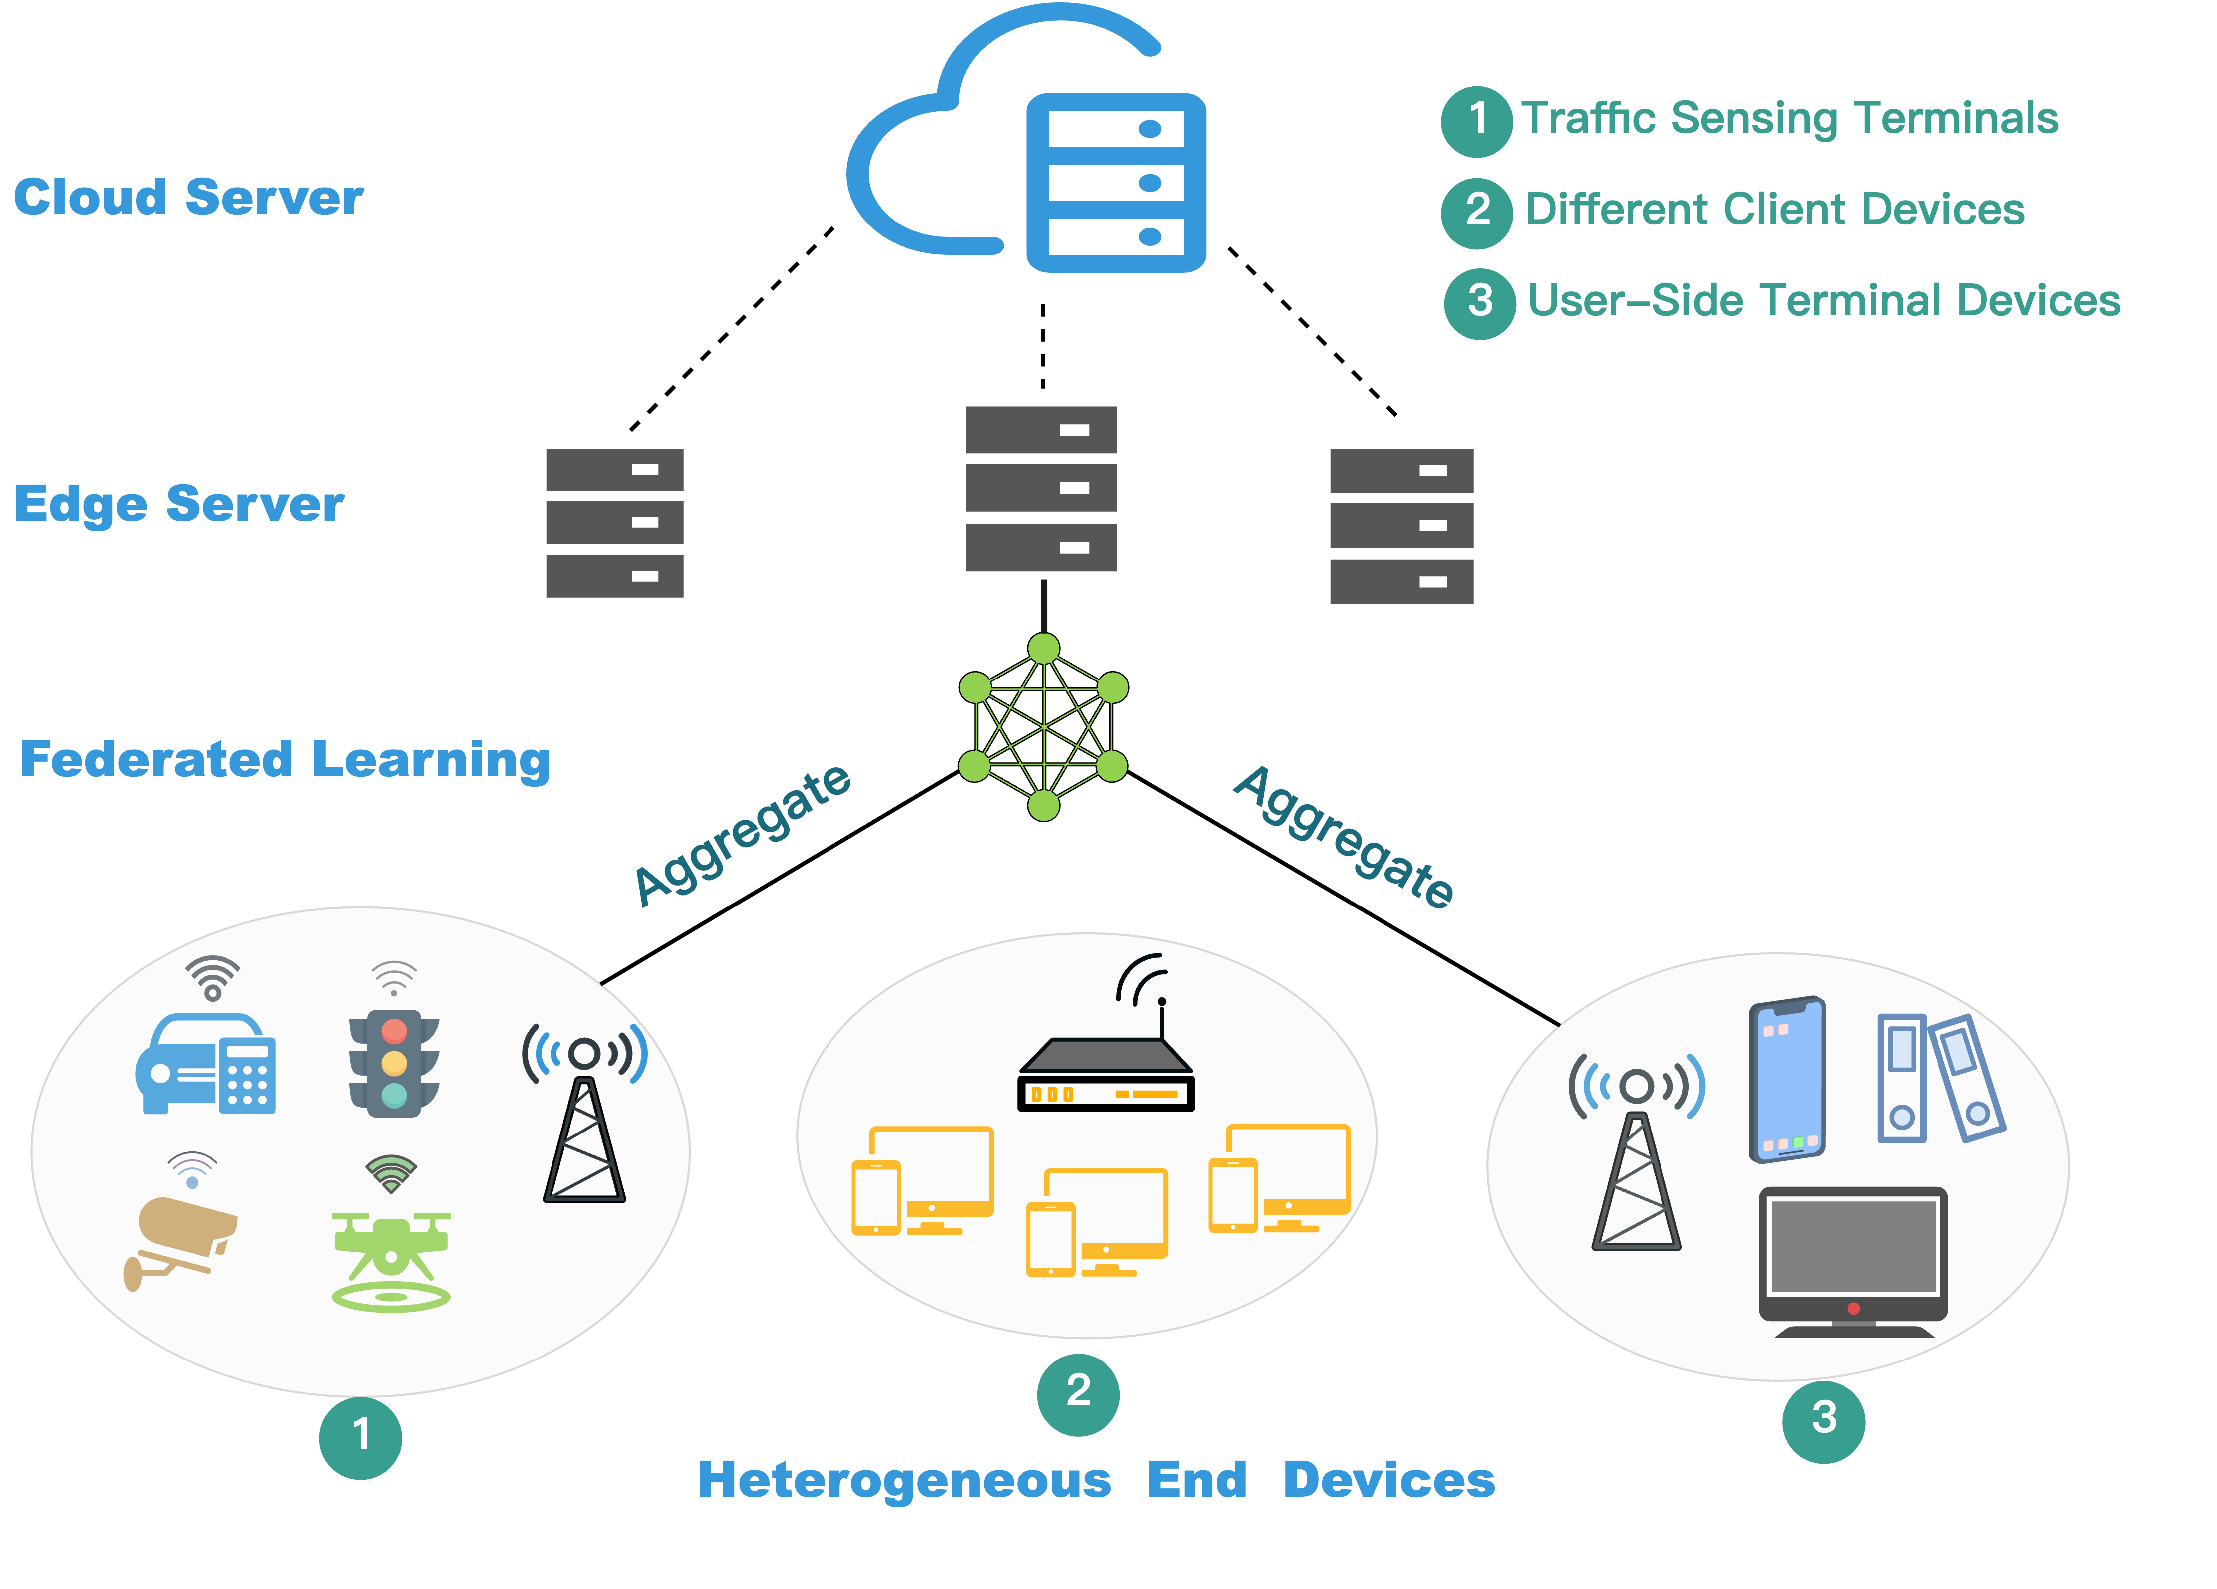
\includegraphics[width=1\linewidth]{IOT-system-new (1).pdf}
    \caption{The non-IID IoT system adopts a cloud-edge-end hierarchical device architecture, which comprises heterogeneous end devices.}
    \label{fig:iot}
\end{figure}

A typical example is the traffic and environmental sensing scenario (Fig. \ref{fig:iot}), where on-board units, traffic signal controllers, surveillance cameras, and unmanned aerial vehicles (UAVs) generate data characterized by distinct category skew and quantity imbalance (e.g., traffic cameras at urban intersections producing far more samples than those in suburban areas). Such heterogeneity poses notable challenges to latency-sensitive tasks like real-time traffic state prediction and signal timing optimization. \rev{Beyond traffic IoT systems, similar data heterogeneity issues persist in other critical industrial tasks reliant on data-driven inference, including load assessment of cylindrical rolling element bearings \cite{shengao11}, fault diagnosis in industrial devices via a neuro-fuzzy approach with hypergraph convolution \cite{shengao12}, and vibration-based gear wear monitoring and prediction techniques \cite{shengao13}—all of which necessitate robust federated learning frameworks capable of handling non-IID data.}

 
Previous research on federated learning has primarily tackled data heterogeneity from three perspectives, each exhibiting limitations in IoT edge scenarios: 
\rev{Firstly, Algorithmic refinements focus on optimizing local training processes \cite{tii-ClientSelectin,iot2} or redesigning global aggregation mechanisms \cite{tii-Spatio–TemporalAware}. However, many of these approaches impose substantial computational or communication overhead, which is often incompatible with the resource limitations of typical IoT edge hardware.
Secondly, Architectural innovations explore advanced model structures (e.g., Vision Transformers \cite{fesvibs}) or novel learning paradigms (e.g., SplitFed \cite{splitfed}) to enhance performance. Nevertheless, such methods frequently depend on specific, non-standardized model architectures or require fundamental changes to the federated learning workflow, hindering their seamless adoption in heterogeneous IoT ecosystems. 
Thirdly, Temporal-spatial explorations investigate patterns like seasonal data fluctuations \cite{tii-Personalized2}, yet they may not adequately address the static, structural heterogeneity inherent in many IoT deployments, such as persistent label and quantity skews across devices. }A critical gap remains: most existing solutions are tailored to mitigate a single type of data skew and lack effective mechanisms to handle the compounded challenges of dual-skewed non-IID data, where both label distribution and sample size vary significantly across clients—a common scenario in real-world IoT systems.


% In this work, we address label distribution skew, quantity skew, and their mixtures in IoT edge environments (Fig. \ref{fig:iot}). We discover client constraint rules based on data distribution dissimilarity and design a client pairing algorithm tailored for resource-limited IoT devices, thereby proposing the Federated Client Pairing and Mutual Constraint (FCPC) framework. Compared to previous non-IID solutions, FCPC requires no network architecture modifications and imposes minimal computational burden, which is necessary for deployment on IoT edge nodes with constrained CPU/memory. Significantly, it enhances accuracy and convergence speed while offering orthogonal compatibility, enabling seamless integration with existing IoT-FL methods.

To overcome these limitations, we introduce the Federated Client Pairing and Mutual Constraint (FCPC) framework, \rev{motivated by a key observation (detailed in Section 4: Motivation): a potential mutual constraint exists among clients and its strength correlates positively with data distribution dissimilarity.} This insight shifts the core challenge to accurately quantifying inter-client data dissimilarity and devising an efficient mechanism to exploit the constraint. FCPC innovates in two aspects. \rev{First, it proposes the Jensen-Shannon Divergence and Skew Indicator Number (JSDN) metric, a novel metric that jointly quantifies label and quantity skews. Second, it employs a JSDN-based client pairing algorithm and injects a pairwise regularization term into local training. FCPC leaves the base model architecture and server aggregation unchanged, while adding a linear-in-parameter local penalty and one partner-model transfer for each paired client; these costs are measured explicitly in the revised evaluation.}



\textbf{Contributions.} The main contributions of this work are summarized as follows:

\begin{itemize}
      \item \textbf{\rev{Novel Insight into Client Constraints:}} A mutual constraint relationship is identified among federated learning clients, with its strength correlating positively with data distribution dissimilarity. A lightweight pairwise regularization mechanism is designed to leverage this relationship, mitigating dimensional collapse in non-IID settings—particularly crucial for IoT edge systems.

    \item \textbf{\rev{Unified Heterogeneity Quantification Metric:}} The JSDN metric is proposed to quantify label and quantity skews within a unified formulation. Providing a more holistic characterization of dual-skewed heterogeneity than single-type metrics, JSDN enables more precise client analysis and pairing.

    \item \textbf{\rev{Plug-and-Play Framework for Practical Deployment:}} We propose the FCPC framework, which does not require core FL algorithms modification. Its design requires no changes to core FL algorithms, operating as an add-on module that introduces only a client pairing step and a lightweight regularization term, thereby enabling practical deployment in heterogeneous IoT environments with minimal integration cost.
    
\end{itemize}





% This paper is structured as follows. Section~\uppercase\expandafter{\romannumeral2} involves related work, and introduces various heterogeneous scenarios in the field of federated learning and the specific details of data heterogeneity. Section~\uppercase\expandafter{\romannumeral3} introduces the federated learning framework and differential privacy.
% Section~\uppercase\expandafter{\romannumeral4} shows the formation of experimental motivation and the gradual deepening process of research ideas through four steps. Section~\uppercase\expandafter{\romannumeral5} describes our system flow. Section~\uppercase\expandafter{\romannumeral6} evaluates the effectiveness of our proposed method and the convenience of seamlessly integrating other algorithms. Section~\uppercase\expandafter{\romannumeral7} summarizes our work and describes the future direction of research.



\section{Related work}

\subsection{ Non-IID IoT Systems}

% The data heterogeneity in federated learning refers to the inconsistent distribution of data between clients, which does not follow the same 、, that is, non independent and identically distributed (non-IID). At present, the mainstream classification methods for data heterogeneity can be divided into three types:

The data heterogeneity in federated learning refers to the inconsistent distribution of data across edge devices, violating the independent and identically distributed (IID) assumption\cite{xiong1}. In IoT ecosystems, this phenomenon intensifies due to device-specific deployment environments and sensing capabilities. Current heterogeneity classification encompasses two dimensions:

At the label level, it is manifested as differences in the label space of the data from each participant, which exerts a profound impact on model training\cite{tii-Heterogeneous}. Divergent label spaces across devices degrade model robustness. Industrial IoT deployments exemplify this issue, where vibration sensors in high-risk manufacturing zones report disproportionate ``equipment failur'' labels, while identical sensors in controlled environments predominantly yield ``normal operation'' labels. 

At the quantity level, this manifests as notable disparities in sample sizes across participants: a single client may possess a vastly larger dataset than the rest, or data volumes may be severely imbalanced among multiple clients.

% Smart city networks demonstrate extreme cases: traffic cameras at urban intersections generate orders of magnitude more samples than particulate matter sensors in peripheral residential zones. This imbalance causes global models to overfit high-data-density devices while underperforming on sparse-data nodes.


\subsection{Existing Solutions}
 % FedAvg\cite{fedavg} , as a pioneering work in the field of federated learning,  aggregates model parameters by weighted averaging. Different from traditional distributed training, FedAvg supports clients to train locally and then upload their local model parameters to the server, which calculates the average of these parameters and weights them according to the amount of data on each device.This approach provides a new way of thinking about distributed learning, but it is a little bit unsatisfactory. For this reason, research on solving the federated learning non-IID problem has gradually emerged in recent years.

\rev{To contextualize our approach, we review prevalent strategies for handling non-IID data and analyze their suitability for dual-skewed IoT scenarios.}

FedProx\cite{fedprox} is an approach designed to address system heterogeneity and data heterogeneity. It enables flexible local computation, which to some extent mitigates the interference caused by resource-constrained federated participants during the training process. At the same time, it merges a proximal term in the loss function to avoid excessive deviation of client training from the global model.

MOON(Model-Contrastive Learning) \cite{moon} mitigates the effects of differences in data distribution by introducing comparative learning techniques into the training process. This method is simple and effective, encouraging model-level feature alignment to improve the performance of federated deep learning models on non-IID datasets. 

% FedAVGM\cite{fedavgm}, which introduces the Momentum mechanism on the basis of FedAvg, can accumulate the information of the previous gradient during the model training process, so that the model can move more smoothly towards the optimal solution when updating the parameters, reduce the oscillation during the training process, and accelerate the convergence speed, which is especially effective in dealing with complex non-convex optimization problems and large-scale datasets. 

\rev{FastPPO\cite{fastppo} proposes an improved PPO-based scheduling algorithm for personalized federated learning in green IoT. By integrating greedy reward allocation and exponential-decay training duration, it adapts to participants’ dynamic resources and preferences, maximizing FL model accuracy while optimizing energy efficiency and participation willingness.}

FedDyn\cite{feddyn} introduces a new approach to construct agent datasets and dynamically extract local knowledge. Instead of using an averaging strategy, it implements focal distillation to emphasize reliable knowledge, effectively solving the problem of knowledge bias.





% \textbf{Summary and Differentiation. }As reviewed, prevailing methods address non-IID challenges through global-model-centric regularization (e.g., FedProx), representation-level alignment (e.g., MOON), or complex knowledge distillation (e.g., FedDyn). While beneficial in certain contexts, these approaches often introduce non-negligible computational overhead or require modifications to the FL protocol, limiting their practicality in standardized, resource-constrained IoT deployments. Crucially, they are primarily designed for single-type skews and lack a direct mechanism to leverage inter-client data dissimilarity. In contrast, our proposed FCPC framework fundamentally diverges by: (1) introducing a pairwise, dissimilarity-aware constraint that actively utilizes data distribution gaps as a convergence driver, (2) operating via a lightweight, plug-and-play regularization term that avoids architectural changes and minimizes overhead, and (3) explicitly targeting the dual-skewed heterogeneity prevalent in IoT edge data through the unified JSDN metric. This positions FCPC as a uniquely practical solution tailored for the dual constraints of statistical heterogeneity and device resource limitations in real-world IoT systems.

\rev{\textbf{Summary and Differentiation. }As reviewed, the prevailing methods tackle non-IID challenges through diverse strategies: global-model-centric regularization (e.g., FedProx), representation-level contrastive learning (e.g., MOON), dynamic knowledge distillation (e.g., FedDyn), trust evaluation for federated learning in mobile network digital twins (e.g., TFL-DT\cite{tfl-dt}), local graph-based aggregation for dual skews (e.g., FBLG\cite{fblg}), causal inference to address aggregation bias (e.g., FedCFA\cite{fedcfa}) and reinforcement learning-based personalized scheduling (e.g., FastPPO). While effective in their specific designs, many require additional local computation or modifications to the core FL protocol. Furthermore, except for FBLG which explicitly targets dual skews, most are primarily designed for or evaluated on single-type heterogeneity and lack an intrinsic mechanism to test whether inter-client dissimilarity is useful for pairing. FCPC differs by: (1) introducing a pairwise constraint selected from quantified label and quantity metadata, (2) leaving server aggregation and model architecture unchanged, and (3) explicitly measuring the computation, storage, and partner-communication costs introduced by this design.}

\rev{\textbf{Security scope and composability. }Recent work demonstrates that statistical-heterogeneity mitigation and Byzantine robustness are distinct requirements. In particular, ScaleSign constructs malicious updates that evade sign-, cosine-, and distance-based filters, while MSGuard combines cosine similarity, sign statistics, and spectral detection to defend against such model-poisoning attacks \cite{yang2025scalesign}. FCPC does not inspect update integrity and therefore must not be interpreted as a poisoning defense. Its paired-model exchange also creates an additional authenticated channel whose reference models should be filtered when adversarial clients are possible. Because FCPC leaves server aggregation unchanged, a Byzantine-robust aggregator or a multi-strategy detector such as MSGuard can be composed with FCPC; evaluating this security--heterogeneity interaction is separated from the honest-client setting studied in the main experiments.}


% In the context of federated learning within IoT systems, the non-IID problem has a significant negative impact on its performance. IoT devices often generate data with varying characteristics due to differences in deployment environments, sensing capabilities, and usage patterns, leading to diverse data distributions. When the data of each IoT device is characterized by a diverse distribution, the updating direction of the model parameters will diverge during the local model training process of each device. This inconsistency in data distribution directly leads to the different directions of local model updating. The increase of this bias seriously hinders the efficient integration of the knowledge extracted from each local model into the global model, which in turn leads to a decrease in the overall performance of federated learning in IoT scenarios.






\section{The System Model and Definitions}
\subsection{Federated Learning Framework}

As a novel machine learning paradigm, federated learning addresses the challenge of training high-performance global models without disclosing local data when multi-source datasets are distributed across different devices or clients. This framework enables model training on decentralized devices (clients) that maintain local datasets without requiring centralized data exchange.

Formally, let $\mathcal{D} = \{D_1, D_2, \ldots, D_n\}$ represent the distributed datasets across $n$ clients, where $D_i$ is the local dataset of client $i$. The objective of federated learning is to train a global model $M$ by aggregating locally computed model updates while minimizing the loss function $\mathcal{L}$ with respect to model parameters $\theta$. This is expressed mathematically as:

\begin{equation}
\min_{\theta} \mathcal{L}(\theta) = \sum_{i=1}^{n} \frac{|D_i|}{|D|} \mathcal{L}_i (\theta),
\label{eq:fl_objective}
\end{equation}
where $|D_i|$ denotes the number of samples in client $i$'s dataset, $|D| = \sum_{i=1}^n |D_i|$ represents the total number of samples across all clients, and $\mathcal{L}_i$ is the loss function computed on the $i$-th client's dataset. This formulation enables effective feature learning from distributed data while ensuring local data residency and privacy preservation.

FedAvg\cite{fedavg} represents a foundational and widely deployed algorithm in federated learning. In FedAvg:
\begin{enumerate}
    \item Each client computes model updates based on local data;
    \item Client updates are transmitted to the central server;
    \item The server aggregates updates via weighted averaging:
    \begin{equation}
    \theta^{(t+1)} = \theta^{(t)} - \eta \sum_{i=1}^{n} \frac{|D_i|}{|D|} \nabla \mathcal{L}_i (\theta^{(t)}).
    \label{eq:fedavg}
    \end{equation}
\end{enumerate}

Where $\theta^{(t)}$ and $\theta^{(t+1)}$ denote the global model parameters updated at time $t$ and after the update, respectively, and $\eta$ denotes the learning rate that controls the magnitude of the update.
% LDP改进版

\subsection{Differential Privacy}

Differential privacy (DP) \cite{dp} provides a rigorous mathematical foundation for privacy preservation in our framework. A randomized mechanism \(\mathcal{M}\) satisfies \(\epsilon\)-differential privacy if: for any two adjacent datasets \(D\) and \(D^{\prime}\) differing by at most one element, and any measurable output set \(S \subseteq \text{Range}(\mathcal{M}):\) 
\begin{equation}
\Pr[\mathcal{M}(D) \in S] \leq e^{\epsilon} \cdot \Pr[\mathcal{M}(D^{\prime}) \in S],
\label{eq:dp_def}
\end{equation}
where \(\epsilon > 0\) is the privacy budget governing the privacy-utility tradeoff. The \(\ell_1\)-sensitivity of a function \(f: \mathcal{D} \rightarrow \mathbb{R}^{k}\) is defined as:
\begin{equation}
\Delta_{1} f = \max_{D \sim D^{\prime}} \|f(D) - f(D^{\prime})\|_{1},
\label{eq:sensitivity}
\end{equation}
where the maximum is taken over all adjacent datasets. The Laplace mechanism achieves \(\epsilon\)-DP by adding sensitivity-scaled noise: \(\mathcal{M}(D) = f(D) + \text{Lap}(\Delta_{1} f / \epsilon)\).

Extending this to federated systems, local differential privacy (LDP) \cite{dpprotocols} enforces privacy directly at the data source. A mechanism \(\mathcal{M}\) satisfies \(\epsilon\)-LDP if, for all pairs of inputs \(v, v' \in \mathcal{D}\) and any output \(y \in \mathcal{Y}\):
\begin{equation}
\frac{\Pr[\mathcal{M}(v) = y]}{\Pr[\mathcal{M}(v') = y]} \leq e^{\epsilon}.
\label{eq:ldp_def}
\end{equation}

This client-side protection eliminates server trust assumptions, aligning with federated learning's core principle of data locality.

In our context, consider client \(k\) reporting a label distribution vector \(h_k \in \mathbb{N}^C\) (where \(C\) is the number of classes) and data size \(N_k \in \mathbb{N}\). The \(\ell_1\)-sensitivities are \(\Delta_1 h_k = 2\) (since changing one sample can affect at most two class counts, e.g., decreasing one count and increasing another) and \(\Delta_1 N_k = 1\) (as a single sample change alters the size by \(\pm 1\)). The LDP perturbation mechanisms are:
\begin{align}
\tilde{h}_k &= h_k + \left(\text{Lap}\left(2 / \epsilon_h\right)\right)^C, \label{eq:ldp_label} \\
\tilde{N}_k &= N_k + \text{Lap}\left(1 / \epsilon_N\right), \label{eq:ldp_size}
\end{align}
where \(\epsilon_h > 0\) and \(\epsilon_N > 0\) denote the privacy budgets allocated to the label distribution and size, respectively.

Through sequential composition, the joint mechanism satisfies \(\epsilon\)-LDP with \(\epsilon = \epsilon_h + \epsilon_N\). To minimize the total variance, the optimal privacy budget allocation is:
\begin{equation}
\epsilon_h^* = \epsilon \cdot \frac{\sqrt{C / N_k}}{\sqrt{C / N_k} + 1}, \quad \epsilon_N^* = \epsilon - \epsilon_h^*, \label{eq:opt_alloc}
\end{equation}
where \(C\) is the class count and \(N_k\) is the local data size. This allocation balances utility between the histogram and scalar protections.



\section{Motivation}
\subsection{Dual Skewed Non-IID Data Leads to Worse Global Model Performance Degradation}
We conduct a preliminary experiment with the classic FedAvg algorithm as an example. We set up 10 clients, record the classification accuracy in three scenarios in the number of 20 global rounds, and draw a line graph, as shown in Fig. \ref{fig:acc vs com}.
It can be observed that a single label distribution skew or quantity skew has been able to roughly learn the data characteristics in the previous rounds of communication. 

% Before 10 rounds of communication, the loss convergence tends to be stable.
% However, in the case of dual skew, FedAvg can only achieve an accuracy of about 85 in 20 rounds of communication, and the convergence of the global model is very unstable.

\begin{figure}[h]
    \centering
    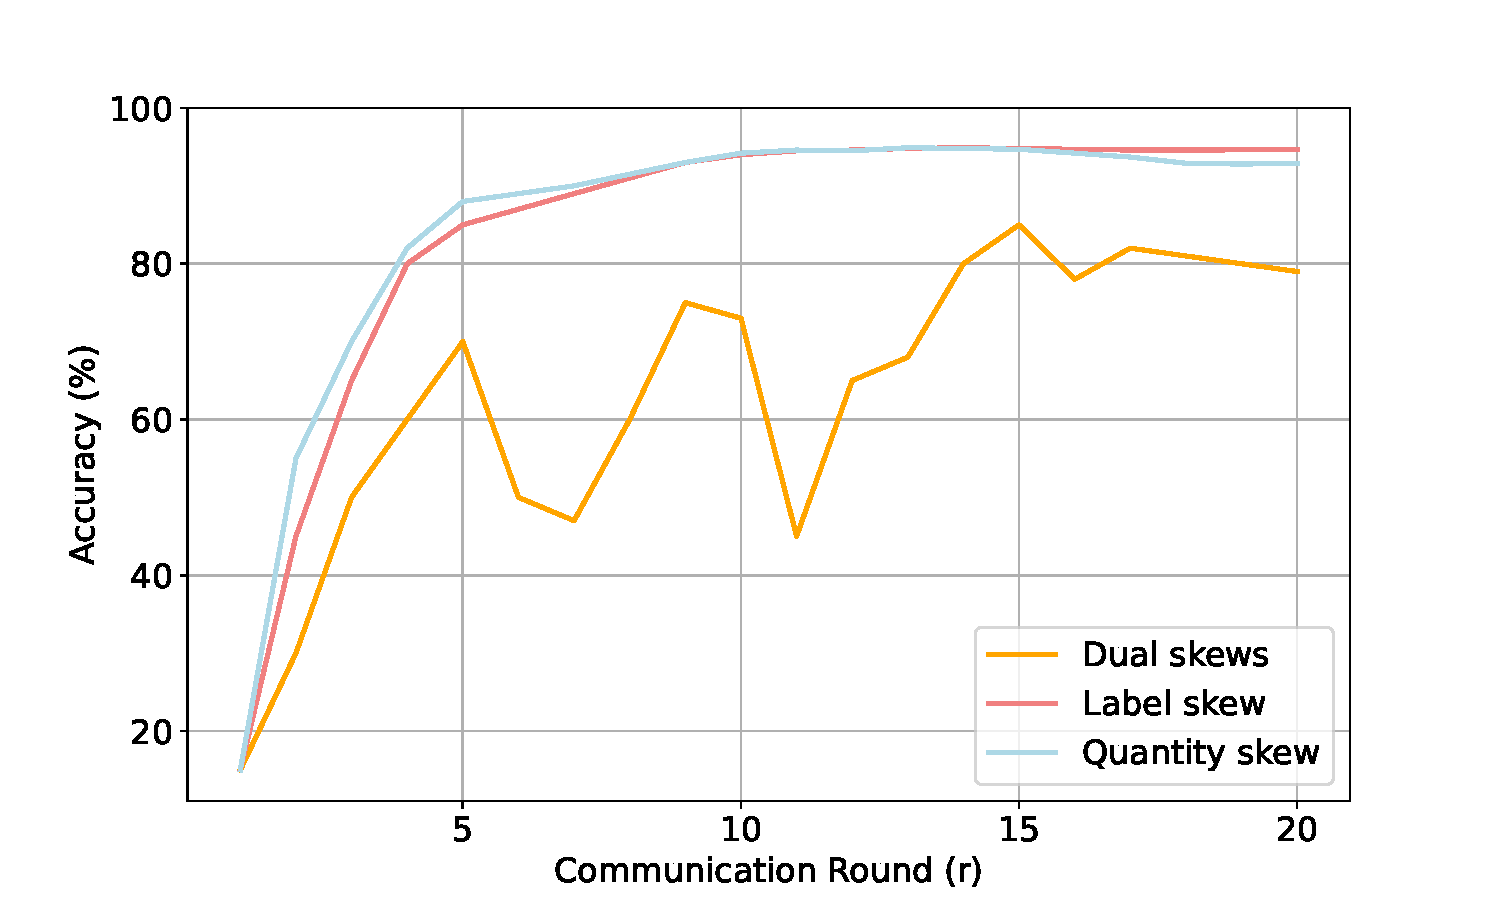
\includegraphics[width=\linewidth]{accuracy_vs_communication_rounds.pdf}
    \caption{Impact of dual skewed non-IID data on global model training induced by heterogeneous label distributions among clients and sample size.}
    \label{fig:acc vs com}
\end{figure}

% \noindent \textbf{Implication 1.} \textit{Compared with the single skew, the dual skewed non-IID data caused by the heterogeneous label distribution and sample size among clients has a greater impact on the performance of the global model.}

\noindent \textbf{Implication 1.} \textit{Compared with the single skew, the dual skewed non-IID data has a greater impact on the performance of the global model.}


\subsection{Deep Understanding of Performance Degradation}
In federated learning, the differences in data distributions across different clients can lead to dimensional collapse in both global and local models, making it difficult for the model to fully utilize the representation space to distinguish between different classes of data, which in turn affects the performance. 

% \noindent \textbf{Implication 2.} \textit{Perhaps we can take a more bottom-up perspective of dimensional collapse to minimise the differences in model updates between participants.}

\noindent \textbf{Implication 2.} \textit{A bottom-up perspective of dimensional collapse may help minimize the differences in model updates between participants.}

\subsection{Discover Potential Constraints Among Participants}

Based on the above study, we consider whether heterogeneous clients can restrict each other to mitigate the low ranking of local models during training. To this end, we conducted simple preliminary experiments. Specifically, we first divided the training samples into 10 slices, each corresponding to the local data of one client. We performed a simple experiment on the probability vector $\mathbf{pc} = (\mathrm{pc}_1, \mathrm{pc}_2, \dots, \mathrm{pc}_K) \sim \text{Dirichlet}(\alpha)$ and assigned the proportion of $\mathrm{pc}_k$ of class $c$ instances to clients $k \in \{1, 2, \dots, K\}$, with $\alpha = 0.01$ to simulate a scenario close to the data heterogeneity in Fig. \ref{fig:demension}.

\begin{figure}[h]
    \centering
    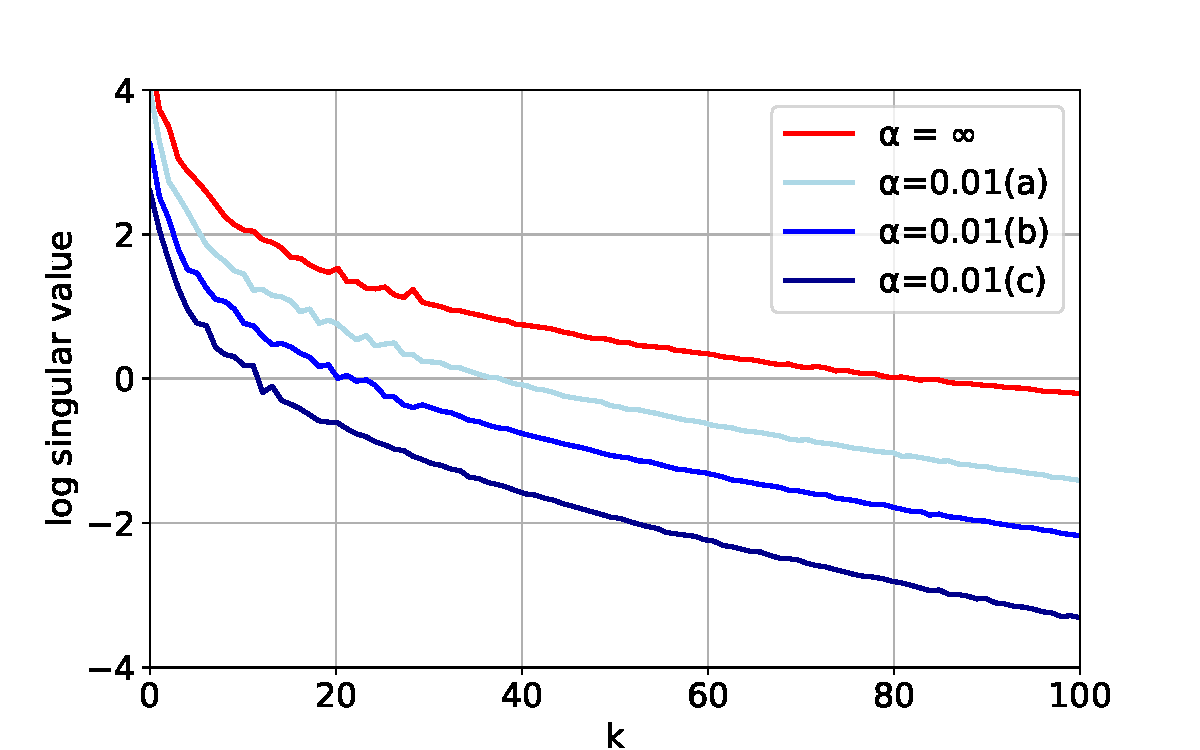
\includegraphics[width=1\linewidth]{demension.pdf}
    \caption{X-axis(k) is the index of the singular values, and y-axis is the logarithm of the singular values. The red lines represent isomorphic scenarios, and the three lines a,b,c represent paired clients with small and relatively large differences and unpaired, respectively. }
    \label{fig:demension}
\end{figure}

\noindent \textbf{Implication 3.} \textit{There appears to be a potential constraint effect that can mitigate the dimensional collapse of local models, and this constraint effect is more pronounced among clients with large differences in data distribution. So we need to quantify these differences precisely.}


\subsection{Promoting Alignment of Model Update Directions Among Participants}

To counteract the effects of non-IID data, FedDecorr\cite{pami} adds a regularization term to the loss function of each local model to encourage tail singularities not to collapse to 0, thus effectively mitigating dimensional collapse.

\noindent \textbf{Implication 4.}  \textit{Inspired by FedDecorr, we propose to optimize the training process by integrating a pairwise-based regularization term. The term acts as a mutual restriction on participants with different data distributions, inducing them to try to maintain the same gradient update direction.}




\section{Proposed Method}
\subsection{Quantify Data Distribution Differences}
After recognizing that the key categories of data heterogeneity are label skew and quantity skew, we design a quantitative metric, JSDN. Specifically, this metric consists of two parts: $\mathcal{JSD}$, which indicates the degree of label skew, and $N$, which indicates the degree of quantity skew.

Jensen-Shannon divergence ($\mathcal{JSD}$) is a measure of similarity between two probability distributions\cite{jsd}. In the federated learning scenario, we choose this metric to measure the similarity of data labeling distributions between different clients. The $\mathcal{JSD}$ value is negatively correlated with the similarity of data distributions, $\mathcal{JSD}$ $\in [0, 1]$. 
In general, the data distribution similarity between clients is inversely proportional to the $\mathcal{JSD}$ value.
In the extreme case, when the  value is 0, it represents that the two sets of data distributions are identical.
The value between two distributions ($ Qa $ ) and ( $Qb$ ) can be formally defined as:

\begin{equation}
\mathcal{JSD}(Q_a,Q_b) = \frac{1}{2} \sum_{i \in \{a, b\}} \mathcal{KL}(Q_i, \mathbb{M}_{ab}),
\end{equation}
where $Q_a$, $Q_b$ are the probability distributions of the data under client $a$ and client $b$, $\mathcal{KL}(\cdot)$ denotes the KLD (Kullback-Leibler Divergence) \cite{kl}. $\mathbb{M}_{ab}$ denotes the mean distribution of $Q_a$ and $Q_b$:
\begin{equation}
\mathbb{M}_{ab} = \frac{Q_a + Q_b}{2}.
\end{equation}

\( N \) is a quantity skew indicator, representing the difference in data volume distribution among clients. When making predictions on new data, the model may not be able to utilize the knowledge learned from other clients well, leading to a decrease in prediction performance. The data quantity difference between client $a$ and $b$ can be quantified by the following normalized indicator:

\begin{equation}
N = \frac{|N_a - N_b|}{N_a + N_b},
\end{equation}
where \( N_a \) and \( N_b \) are the data volumes of clients \( a \) and \( b \), respectively. This equation calculates the normalized value of the difference in data volume between two clients, with \( N \in [0, 1] \). The equation for JSDN is given by:
 
\begin{equation}
JSDN = (1-\lambda)\mathcal{JSD} + \lambda {N}.
\end{equation}

In Eq.(12), \(\lambda\) is a weighting parameter that allows us to adjust the influence of data volume skew relative to label skew. This adjustment is essential, as label skew and volume skew typically have different degrees of impact on the federated learning system's performance. By tuning \(\lambda\), we can balance the contributions of these two factors in the overall measure of data heterogeneity.

\subsection{Client Pairing Algorithm}
\subsubsection{Data Upload and JSDN Matrix Generation}

We assume $n$ clients participate in federated training, each with a dataset corresponding to category $C$. Before local training begins, each client will first add data perturbations to the local label distribution and data size through LDP, and then upload the processed results to the server. Based on the differential privacy, we have determined a equation that integrates privacy and performance coefficients. The privacy budget allocated to label distribution and data size will be adaptively adjusted according to $n$ and $C$. The input for the corresponding JSDN calculation becomes the LDP processed $\hat{\mathbf{p}}$ and  $\hat{N}$. Specifically, for client $i$ and client $j$, the calculated JSDN value is denoted as \(J_{ij}\). Combining all the \(J_{ij}\) together forms an $n$-dimensional JSDN matrix. This matrix provides the basis for the subsequent client pairing.





% \begin{algorithm}
% \SetAlgoLined
% \caption{LDP for Federated Statistics}
% \label{alg:ldp_fl}
% \SetKwProg{Fn}{Function}{:}{end}
% \SetKwInOut{Input}{Input}
% \SetKwInOut{Output}{Output}

% % ====== Phase 1: Client-side LDP Encryption ======
% \Fn{ClientLDP($h_k, n_k, C$)}{
%     \Input{Local label distribution $h_k = [c_1, \dots, c_C]^\top$\ ,
%            Local data size $n_k$ ,
%            Number of classes $C$}
%     \Output{Perturbed statistics $(\tilde{h}_k, \tilde{n}_k)$}
    
%     $\tilde{h}_k \gets \text{zeros}(C)$\;
%     \For{$j \gets 1$ \KwTo $C$}{
%         $\eta_j \sim \text{Laplace}(0, 2/\epsilon_h)$\;
%         $\tilde{c}_j \gets \max(0, c_j + \eta_j)$\;
%         $\tilde{h}_k[j] \gets \tilde{c}_j$\;
%     }
%     $\zeta \sim \text{Laplace}(0, 1/\epsilon_N)$\;
%     $\tilde{n}_k \gets n_k + \zeta$\;
%     \Return $(\tilde{h}_k, \tilde{n}_k)$\;
% }

% % ====== Phase 2: Server-side Parsing ======
% \Fn{ServerParse($\{(\tilde{h}_k, \tilde{n}_k)\}_{k=1}^M, C$)}{
%     \Input{Perturbed statistics $\{(\tilde{h}_k, \tilde{n}_k)\}_{k=1}^M$\\
%            Number of classes $C$}
%     \Output{Aggregated distribution $\hat{\mathbf{p}}$, Total size $\hat{N}$}
    
%     $\hat{\mathbf{p}} \gets \mathbf{0}^C$\;
%     $\hat{N} \gets 0$\;
%     \For{$k \gets 1$ \KwTo $M$}{
%         $\hat{\mathbf{p}} \gets \hat{\mathbf{p}} + \tilde{h}_k$\;
%         $\hat{N} \gets \hat{N} + \tilde{n}_k$\;
%     }
%     $\hat{\mathbf{p}} \gets \hat{\mathbf{p}} / \|\hat{\mathbf{p}}\|_1$\;
%     \Return $(\hat{\mathbf{p}}, \hat{N})$\;
% }
% \end{algorithm}





\subsubsection{Client Pairing Process}
% When the number of clients $n$ is even, we pair all clients into $n/2$ pairs. We start from the original JSDN matrix, which records the JSDN values between all pairs of clients.
% Traverse the JSDN matrix and identify its maximum value \(J_{max}\). Suppose its corresponding subscripts are $i$ and $j$. This means that the data distribution difference between client $i$ and client $j$ is the largest.
% Then, set all elements in the $i$-th row and $j$-th row, and the $i$-th column and $j$-th column of the matrix (except the diagonal elements) to zero. In the updated matrix, find the maximum value \(J_{mn}\) again, and pair the corresponding clients m and n as the second group. Repeat this process, updating the matrix after each pairing until all clients are paired, and finally obtaining \(n/2\) pairs of clients.
% The core idea of this pairing method is to preferentially pair clients with large data distribution differences together because the constraint relationship between clients with larger differences may be stronger.

\rev{When the number of clients $n$ is even, we pair all clients into $n/2$ pairs, starting from the original JSDN matrix that records the JSDN values between all client pairs. We first traverse the JSDN matrix to identify its maximum value $J_{\text{max}}$, with the corresponding row and column subscripts denoted as $i$ and $j$. This indicates that the data distribution difference between client $i$ and client $j$ is the largest across all pairs.
Subsequently, we set all elements in the $i$-th row, $j$-th row, $i$-th column and $j$-th column of the matrix (excluding the diagonal elements) to zero. For the updated matrix, we again identify the maximum JSDN value and pair the corresponding clients as the second group. This process is repeated iteratively: after each pairing operation, the corresponding rows and columns of the paired clients in the matrix are zeroed out, until all clients are paired. Finally, we obtain $n/2$ client pairs in total.}
The core idea of this pairing method is to prioritize pairing clients with large data distribution differences together. This is because the constraint relationship between clients with greater distribution differences tends to be stronger.


% \begin{algorithm}
% \SetAlgoLined
% \caption{Client Pairing}
% \label{alg:client_pairing}
% \SetKwInOut{Input}{Input}
% \SetKwInOut{Output}{Output}

% \Input{Label distributions $\hat{\mathbf{p}}= \{\hat{\mathbf{p_1}},\hat{\mathbf{p_2}}, \dots, \hat{\mathbf{p_n}}\}$, \\
%         Data sizes $\hat{N} = \{\hat{N_1}, \hat{N_2}, \dots,\hat{N_n} \}$, \\
%         Number of clients $n$}
% \Output{Client pairing set $P_{\text{pairs}}$}

% Initialize similarity matrix $J \gets \text{zeros}(n \times n)$ \\
% \For{$i \gets 1$ \KwTo $n$}{
%     \For{$j \gets i+1$ \KwTo $n$}{
%         $J_{ij} \gets \text{JSDN}(\hat{\mathbf{p_i}},\hat{\mathbf{p_j}};\hat{N_i},\hat{N_j})$ \\
%         $J_{ji} \gets J_{ij}$ 
%     }
% }

% $P_{\text{pairs}} \gets \emptyset$ \\
% \eIf{$n$ is even}{
%     \For{$k \gets 1$ \KwTo $n/2$}{
%         $(i^*, j^*) \gets \underset{i,j}{\arg\max} \, J_{ij}$ \\
%         $P_{\text{pairs}} \gets P_{\text{pairs}} \cup \{(i^*, j^*)\}$ \\
%         \For{$x \gets 1$ \KwTo $n$}{
%             $J_{i^*x} \gets 0, \, J_{j^*x} \gets 0$ \\
%             $J_{xi^*} \gets 0, \, J_{xj^*} \gets 0$
%         }
%     }
% }{
%     \For{$k \gets 1$ \KwTo $(n - 1)/2$}{
%         $(i^*, j^*) \gets \underset{i,j}{\arg\max} \, J_{ij}$ \\
%         $P_{\text{pairs}} \gets P_{\text{pairs}} \cup \{(i^*, j^*)\}$ \\
%         \For{$x \gets 1$ \KwTo $n$}{
%             $J_{i^*x} \gets 0, \, J_{j^*x} \gets 0$ \\
%             $J_{xi^*} \gets 0, \, J_{xj^*} \gets 0$
%         }
%     }
% }
% \Return $P_{\text{pairs}}$
% \end{algorithm}



\begin{algorithm}
\SetAlgoLined
\caption{Client Pairing}
\label{alg:client_pairing}
\SetKwInOut{Input}{Input}
\SetKwInOut{Output}{Output}

\Input{Label distributions $\hat{\mathbf{p}}=\{\hat{\mathbf{p}}_1,...,\hat{\mathbf{p}}_n\}$, Data sizes $\hat{N}=\{\hat{N}_1,...,\hat{N}_n\}$, Clients $n$}
\Output{Pairing set $P_{\text{pairs}}$}

Initialize $J \gets \text{zeros}(n \times n)$ \\
\For{$i \gets 1$ \KwTo $n$}{
    \For{$j \gets i+1$ \KwTo $n$}{$J_{ij}=J_{ji}=\text{JSDN}(\hat{\mathbf{p}}_i,\hat{\mathbf{p}}_j;\hat{N}_i,\hat{N}_j)$}
}

$P_{\text{pairs}} \gets \emptyset$ \\
\eIf{$n$ even}{
    \For{$k \gets 1$ \KwTo $n/2$}{
        $(i^*,j^*) \gets \arg\max J_{ij}$, $P_{\text{pairs}} \cup=\{(i^*,j^*)\}$ \\
        \For{$x \gets 1$ \KwTo $n$}{$J_{i^*x}=J_{j^*x}=J_{xi^*}=J_{xj^*}=0$}
    }
}{
    \For{$k \gets 1$ \KwTo $(n-1)/2$}{
        $(i^*,j^*) \gets \arg\max J_{ij}$, $P_{\text{pairs}} \cup=\{(i^*,j^*)\}$ \\
        \For{$x \gets 1$ \KwTo $n$}{$J_{i^*x}=J_{j^*x}=J_{xi^*}=J_{xj^*}=0$}
    }
}
\Return $P_{\text{pairs}}$
\end{algorithm}


When $n$ is odd, we can only form $(n - 1)/2$ pairs of clients, and there will be one client left at the end. In this case, the minimum value in the JSDN matrix represents that the data distribution difference between this client and other clients is relatively small. From the perspective of data distribution, this client is roughly in the middle position of the client distribution. That is to say, its label distribution and data volume are representative to a certain extent within the overall client cohort, and its discrepancies from other clients are less pronounced than those between certain other client pairs. Therefore, we choose to abandon the client corresponding to the minimum value in the JSDN matrix to avoid the interference of the parity of the number of federated learning participants on the pairing process, thus simplifying the pairing process and improving the adaptability of the pairing algorithm.


\subsection{FCPC}

\begin{figure*}[htbp]
    \centering
    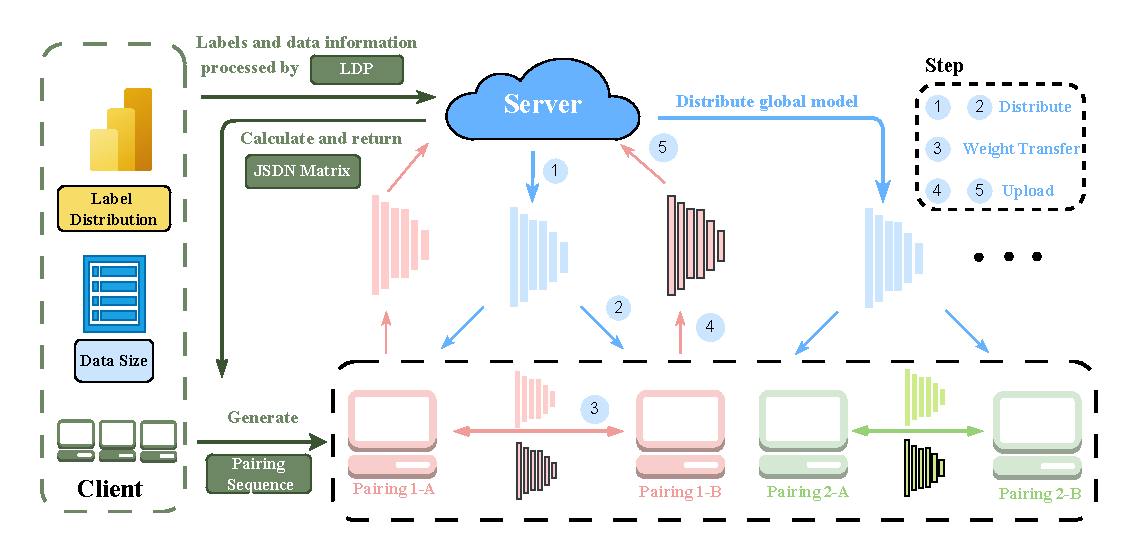
\includegraphics[width=0.8\textwidth]{FCPC.drawio (2).drawio.pdf}
    \caption{Framework of FCPC. The left part demonstrates the process that participants in federated learning upload the label distribution and data size to the server after local differential privacy (LDP) processing. The server then calculates the JSDN matrix and returns the pairing sequence. The right part shows the pairing training process of the participants. Taking the red client pair as an example: the server initializes the global model and distributes it to the clients (Steps 1 and 2). At the end of each training round, between the client pairs, the local weights need to be uploaded to the paired client as a constraint term for the client in the next round (Step 3). Meanwhile, the weights are uploaded to the server for global aggregation (Steps 4 and 5).}
    \label{fig:FCPC}
\end{figure*}

Motivated by the above observation and analysis of the potential constraints between heterogeneous clients in federated learning, we explore how to fully utilize such constraints to mitigate the impact of data heterogeneity during federation training.
During the original federation training, clients train individually with their local datasets and finally upload the model weights to the central server for federated averaging, during this period, the clients cannot perceive the data distribution gaps with other clients, and even if mutual constraints exist, they cannot achieve the constraint effect. Therefore, we propose to mitigate this problem by including constraints during local training. A natural way to achieve this is to add the following regularization term to the loss function during training. The system architecture is shown in Fig. \ref{fig:FCPC}. Formally, the proposed regularization term is defined as:

\begin{equation}
L_{\text{FCPC}}(w_k, X) = \|w_k^t- w_{k'}^{t-1}\|^2 ,
\end{equation}
where \( w_k^t \) represents the local weight of client $k$ in $t$-round training and \( w_{k'}^{t-1}\) represents the weight of the client paired with client $k$ in the $(t-1)$-th round of training.
At each round, a subset $K$ of the total devices is selected to train. The total communication round is $T$ (As shown in Algorithm \ref{alg:FCPC}).

Each client $k$ is selected with probability $p_k$ (a weight coefficient that quantifies the proportional contribution of its local data to the global model), where $p_k \geq 0$ and $\sum_{k=1}^n p_k = 1$. This coefficient is calculated as $p_k = N_k / N_{\text{total}}$, with $N_k$ denoting the data volume of client $k$ and $N_{\text{total}} = \sum_{k=1}^n N_k$ representing the total data volume across all $n$ clients.

After each round of local training, the clients will send the local training weights to the server and the paired clients. The weights sent to the server are used for global aggregation, and the portion sent to the paired clients is used for constructing constraints for the next round of local training for the paired clients. The overall objective of each local client is

\begin{equation}
\min_{w} \ell(w, X, \mathbf{y}) + \beta L_{\text{FCPC}}(w, X),
\label{equa:beta}
\end{equation}
where \(\ell\) is the cross entropy loss, and $\beta$ is the regularization coefficient of FCPC. Essentially, $L_{\text{FCPC}}$ penalizes the difference between the paired clients, thus preventing the two from going in opposite directions of gradient updating during training. Instead, it constrains the paired clients so that they try to maintain the same direction of gradient updating, speeding up model convergence. This regularization term solves the statistical heterogeneity problem by restricting the local updates of the heterogeneous clients without requiring manually set the number of local epochs. We summarize the steps of FCPC in Algorithm \ref{alg:FCPC}.

In addition, the Appendix provides boundedness and single-skew properties of JSDN, a standard nonconvex stationarity result for the frozen-reference local objective, a $1/2$ approximation guarantee for greedy maximum-dissimilarity matching, and exact complexity and communication accounting.
%s算法




\begin{algorithm}[h]
\SetAlgoLined
\caption{FCPC (Proposed Framework)}
\label{alg:FCPC}
\SetKwInOut{Input}{Input}
\SetKwInOut{Output}{Output}
\Input{$K$, $T$, $\beta$, $w^0$, $n$, $p_k$ for $k = 1, \dots, n$}
\Output{Optimized model $w^T$}

\For{$t \gets 0$ \KwTo $T - 1$}{
    $S_t \gets$ random subset of $K$ devices
    

    Send $w^t$ to all $k \in S_t$ \\
    \ForEach{device $k \in S_t$}{
        Find $w_k^{t + 1} \approx \arg \min_{w} \left[ \ell(w; X, \mathbf{y}) + \beta \|w_k^t - w_{k'}^{t - 1}\|^2 \right]$
    }
    \ForEach{device $k \in S_t$}{
        Send $w_k^{t + 1}$ to server
    }
    $w^{t + 1} \gets \frac{1}{|S_t|} \sum_{k \in S_t} w_k^{t + 1}$
}
\Return $w^T$
\end{algorithm}




\section{Performance Analysis}

\subsection{Experimental Setups}
In our experimental setup, all participants actively participated in each round of the training process. For network architecture, we used ResNet18\cite{resnet} and MobileNetV2 \cite{mobilenetv2}, respectively. We performed 100 rounds of communication for all experiments on the CIFAR10/100\cite{cifar10} datasets. Both CIFAR10 and CIFAR100 have 50, 000 training samples and 10,000 test samples, and the size of each image is 32$\times$32. 

Local training was performed for 10 epochs in each round of communication using the SGD optimizer with a learning rate of 0.01 and a batch size of 64. In addition, we applied data enhancement to all experiments.




% \begin{table*}[htbp]
% \caption{Test Accuracy on MNIST and FEMNIST Under Single Types of Non-IID Scenarios}
% \label{tab:single}
% \centering
% \footnotesize
% \begin{tabular}{@{}l l c c c c c@{}}
% \toprule
% Non-IID Scenarios & Dataset & FCPC & FedAvg & FedProx & FedDyn & MOON \\
% \midrule
% \multirow{2}{*}{Label distribution skew} 
%     & MNIST   & \textbf{98.15} & 97.32 & 97.96 & 97.48 & 97.54 \\
%     & FEMNIST & \textbf{97.34} & 96.35 & 96.28 & 97.09 & 96.56 \\
% \addlinespace[0.5ex]  % 增加行间距
% \multirow{2}{*}{Quantity skew} 
%     & MNIST   & \textbf{98.28} & 97.18 & 97.78 & 97.63 & 97.65 \\
%     & FEMNIST & \textbf{97.24} & 95.97 & 96.37 & 96.52 & 96.36 \\
% \bottomrule
% \end{tabular}
% \end{table*}




% \begin{table}[htbp]
% \caption{Performance Comparison Under Different Level of Dual Skewed Non-IID Data Settings on CIFAR10 and CIFAR100 Datasets}
% \label{tab:dual}
% \centering
% \footnotesize
% \begin{tabular}{lcccccc}
% \toprule
% Dataset & \multicolumn{3}{c}{CIFAR10} & \multicolumn{3}{c}{CIFAR100} \\ 
% \cmidrule(lr){2-4} \cmidrule(lr){5-7}
% Method / $\alpha$ & 0.05 & 0.1 & 0.5 & 0.05 & 0.1 & 0.5 \\ 
% \midrule
% FedAvg \textcolor{blue}{(AISTATS, 2017)} & 53.74 & 65.19 & 79.98 & 49.76 & 56.43 & 61.59 \\ 
% FedProx \textcolor{blue}{(MLsys, 2020)}  & 53.21 & 65.20 & 79.46 & 50.22 & 56.37 & 61.59 \\ 
% MOON \textcolor{blue}{(CVPR, 2021)}      & 59.68 & 67.60 & 80.04 & 45.68 & 56.37 & 61.81 \\ 
% FedDyn \textcolor{blue}{(ICPADS, 2023)}  & 62.24 & 68.49 & 77.38 & 49.73 & 56.36 & 61.28 \\ 
% FBLG \textcolor{blue}{(IJCAI, 2024)}     & 62.95 & 69.13 & 79.82 & 50.45 & 57.62 & 61.28 \\ 
% \midrule
% \textbf{FCPC}          & \textbf{63.17} & \textbf{70.59} & \textbf{80.28} & \textbf{52.53} & \textbf{58.12} & \textbf{62.72} \\
% \bottomrule
% \end{tabular}
% \end{table}




\subsection{Performance Under Single Types of Non-IID Scenarios}

We selected two small and medium-sized datasets, MNIST\cite{MNIST} and FEMNIST, and carried out a detailed study on the accuracy of the FCPC algorithm in single-type non-IID scenarios.
During the experiment, we simulated two common single-type non-IID conditions in Table \ref{tab:single}: label distribution skew and quantity skew. 

For the situation of label distribution skew, the results show that FCPC achieves an accuracy of 0.9815 on the MNIST dataset and an accuracy of 0.9734 on the FEMNIST dataset. In comparison, the performance of other methods on these two datasets is relatively weak. This fully demonstrates that when dealing with data with label distribution skew, FCPC can more effectively mine the feature information in the data, improve the model's recognition ability for different types of data, and thus obtain higher accuracy.



\begin{table}[h]        % 注意这里是 table，不是 table*，表示放在单栏内
\caption{Test Accuracy on MNIST and FEMNIST Under Single Types of Non-IID Scenarios}
\label{tab:single}
\centering
\footnotesize
\resizebox{\linewidth}{!}{ % 关键：将表格缩放至当前栏宽度
\begin{tabular}{@{}l l c c c c c@{}}
\toprule
Non-IID Scenarios & Dataset & FCPC & FedAvg & FedProx & FedDyn & MOON \\
\midrule
\multirow{2}{*}{Label distribution skew} 
    & MNIST   & \textbf{98.15} & 97.32 & 97.96 & 97.48 & 97.54 \\
    & FEMNIST & \textbf{97.34} & 96.35 & 96.28 & 97.09 & 96.56 \\
\addlinespace[0.5ex]
\multirow{2}{*}{Quantity skew} 
    & MNIST   & \textbf{98.28} & 97.18 & 97.78 & 97.63 & 97.65 \\
    & FEMNIST & \textbf{97.24} & 95.97 & 96.37 & 96.52 & 96.36 \\
\bottomrule
\end{tabular}
}
\end{table}

In the experimental scenario of quantity skew, FCPC also demonstrates excellent performance. On the MNIST dataset, the accuracy of FCPC reaches 0.9828, and on the FEMNIST dataset, it is 0.9724. It can be seen that when facing the situation of large differences in data quantity, FCPC can still maintain a high accuracy, effectively avoiding the problem of model performance degradation caused by data imbalance.





\subsection{Performance Under Dual Types of Non-IID Scenarios}
% However, recent studies have pointed out that it is much more difficult to handling mixed types of data skews in federated learning than single types, as the heterogeneity of different types of data tends to create potential bundling effects. Therefore, we also evaluated the performance of the FCPC algorithm in a mixed scenario of skewed label and quantity distributions on the CIFAR10 dataset. We set up two mixed heterogeneous distribution scenarios with different degrees of $\alpha$ = 0.05 and 0.5, respectively, for verifying the performance of FCPC under extreme data heterogeneity and general data heterogeneity distributions.

% The experimental results, as shown in the table, show that FCPC leads the way with an accuracy of 0.6426 and 0.8826, respectively, while the accuracy of other methods decreases substantially. 


Addressing mixed types of data skews (e.g., concurrent label and quantity skews) is recognized as a significantly more challenging task in federated learning than handling single-type skews, as the interplay between different heterogeneities can lead to compounded performance degradation. To evaluate the efficacy of FCPC under such complex conditions, experiments were conducted on the CIFAR-10 dataset under dual-skew scenarios. The degree of heterogeneity was controlled using a Dirichlet distribution parameter $\alpha \in \{0.05, 0.1, 0.5\}$, simulating environments with extreme, high, and moderate data heterogeneity, respectively.

Experimental results, summarized in Table \ref{tab:dual}, demonstrate that the proposed FCPC framework consistently achieves superior classification accuracy across all tested heterogeneity levels. In contrast, the performance of all baseline methods exhibits a more substantial decline, particularly under the extreme heterogeneity condition ($\alpha=0.05$).

\begin{table}[htbp]
\caption{Performance Comparison Under Different Levels of Dual-Skewed Non-IID Data on CIFAR-10 and CIFAR-100}
\label{tab:dual}
\centering
\scriptsize  % 进一步缩小字体，原为 \footnotesize
\resizebox{\linewidth}{!}{ % 自动缩放表格宽度至当前栏可用宽度
\begin{tabular}{lcccccc}
\toprule
Dataset & \multicolumn{3}{c}{CIFAR10} & \multicolumn{3}{c}{CIFAR100} \\ 
\cmidrule(lr){2-4} \cmidrule(lr){5-7}
Method / $\alpha$ & 0.05 & 0.1 & 0.5 & 0.05 & 0.1 & 0.5 \\ 
\midrule
FedAvg \textcolor{blue}{(AISTATS, 2017)} & 53.74 & 65.19 & 79.98 & 49.76 & 56.43 & 61.40 \\ 
FedProx \textcolor{blue}{(MLsys, 2020)}  & 53.21 & 65.20 & 79.46 & 50.22 & 56.37 & 61.59 \\ 
MOON \textcolor{blue}{(CVPR, 2021)}      & 59.68 & 67.60 & 80.04 & 45.68 & 56.37 & 61.81 \\ 
FedDyn \textcolor{blue}{(ICPADS, 2023)}  & 62.24 & 68.49 & 77.38 & 49.73 & 56.36 & 61.28 \\ 
FBLG \textcolor{blue}{(IJCAI, 2024)}     & 62.95 & 69.13 & 79.82 & 50.45 & 57.62 & 61.38 \\ 
\rev{FedCFA}\textcolor{blue}{(AAAI, 2025)}     & \rev{63.15} & \rev{69.83} & \rev{80.45} & \rev{51.47} & \rev{57.81} & \rev{62.13} \\ 
\midrule
\textbf{FCPC}          & \textbf{63.17} & \textbf{70.59} & \textbf{80.28} & \textbf{52.53} & \textbf{58.12} & \textbf{62.72} \\
\bottomrule
\end{tabular}
}
\end{table}



\subsection{ Orthogonality of FCPC with Existing FL Algorithms}

Thanks to the regularization property of FCPC method, it acts on the local training stage through pairing between devices. It only needs to introduce the pairing algorithm on the basis of other existing methods and add an additional term $L_{\text{FCPC}}$ on the loss function. In addition, it does not need any change, which makes FCPC have the natural advantage of plug-and-play.

To validate this orthogonality, FCPC is integrated into five representative baseline algorithms, namely FedAvg\cite{fedavg}, FedProx\cite{fedprox}, MOON\cite{moon}, FBLG\cite{fblg}, and FedCFA\cite{fedcfa}. Two sets of experiments are conducted: (1) CIFAR-10 dataset with the ResNet-18 model, where data are partitioned among 10 clients; \rev{ (2) TinyImageNet dataset with the same client partitioning strategy. The degree of heterogeneity is quantified using a Dirichlet distribution with \( \alpha \in \{0.05, 0.1, 0.5\} \) (smaller \( \alpha \) indicates stronger heterogeneity). The experimental objective is to verify whether integrating FCPC can enhance the performance of baseline methods under varying non-IID degrees.}



Experimental results indicate that embedding FCPC as a regularization term into baseline algorithms yields notable performance gains, especially under strongly heterogeneous settings (\( \alpha = 0.05 \) and \( \alpha = 0.1 \)). On the CIFAR-10 dataset, the performance improvement ranges from approximately 4.0\% to 9.4\% compared with the original baselines. For instance, FedAvg achieves 53.74\% accuracy when \( \alpha = 0.05 \), and the accuracy increases to 63.17\% after integrating FCPC, representing a 9.43\% improvement. \rev{On the TinyImageNet dataset, the improvement under \( \alpha = 0.05 \) and \( \alpha = 0.1 \) is about 5.0\% and 3.5\%–4.5\%, respectively.  }

% The experimental results in Table \ref{tab:add FCPC} demonstrate the effectiveness of integrating the FCPC algorithm with other FL algorithms, which suggests a substantial enhancement in its handling of non-IID data.

\rev{The results presented in Tables \ref{tab:add FCPC} and \ref{tab:tinyimagenet} collectively demonstrate the effectiveness and orthogonality of integrating FCPC with existing FL algorithms. Notably, FCPC consistently enhances the performance of baseline methods across different datasets and heterogeneity levels, which verifies its ability to strengthen the non-IID data handling capability of FL frameworks.}



\begin{table*}[htbp]
\caption{Orthogonality Analysis of FCPC Integration With Existing FL Algorithms (ResNet-18, CIFAR10)}
\label{tab:add FCPC}
\centering
\footnotesize
\setlength{\tabcolsep}{4pt} % 紧凑列间距
\begin{tabular}{@{}l *{5}{c c} c@{}}
\toprule
\textbf{$\alpha$}  & \multicolumn{2}{c}{FedAvg} & \multicolumn{2}{c}{FedProx} & \multicolumn{2}{c}{MOON} & \multicolumn{2}{c}{FBLG}  & \multicolumn{2}{c}{FedCFA}\\
& \multicolumn{2}{c}{\textcolor{blue}{\scriptsize (AISTATS 2017)}} & \multicolumn{2}{c}{\textcolor{blue}{\scriptsize (MLsys 2020)}} & \multicolumn{2}{c}{\textcolor{blue}{\scriptsize(CVPR 2021)}} & \multicolumn{2}{c}{\textcolor{blue}{\scriptsize(IJCAI 2024)}}  & \multicolumn{2}{c}{\textcolor{blue}{\scriptsize(AAAI 2025)}}\\
\cmidrule(lr){2-3} \cmidrule(lr){4-5} \cmidrule(lr){6-7} \cmidrule(lr){8-9} \cmidrule(lr){10-11}
& Orig. & \textbf{\scriptsize +FCPC} & Orig. & \textbf{\scriptsize +FCPC} & Orig. &\textbf{\scriptsize +FCPC} & Orig. & \textbf{\scriptsize +FCPC} & Orig. & \textbf{\scriptsize +FCPC} \\
\midrule
\textbf{0.05} & 53.74 & 63.17 & 53.21 & 61.29 & 59.68 & 63.46  & 62.95 & 63.08 & 63.15 & \textbf{64.23} \\
\textbf{0.1}  & 65.19 & 70.59 & 65.20 & \textbf{72.83} & 67.60 & 72.26  & 69.13 & 70.45 & 69.83 & 72.29\\
\textbf{0.5}  & 79.98 & 80.28 & 79.46 & 80.35 & 80.04 & 80.82 & 79.82 & 80.83  & 80.45 &\textbf{81.62}  \\
\bottomrule
\end{tabular}

\end{table*}








% \begin{table}[!t]
% \centering
% \footnotesize % 字号缩小 适配IEEE双栏
% \caption{Orthogonality Analysis of FCPC Integration With Existing FL Algorithms (TinyImageNet)}
% \label{tab:tinyimagenet}

% \begin{tabular}{lD{.}{.}{2.2}D{.}{.}{2.2}D{.}{.}{2.2}}
% \toprule
% Method & \multicolumn{3}{c}{TinyImageNet} \\ % 补回丢失的这一行核心表头
% \cmidrule(lr){2-4}  % 表头下方短横线，左右留白更美观
%        & \textbf{$\alpha = 0.05$ }&\textbf{ $\alpha = 0.1$} &\textbf{ $\alpha = 0.5$} \\
% \midrule
% FedAvg {\textcolor{blue}{\scriptsize (AISTATS 2017)}        & 35.48 & 39.53 & 46.97 \\
% \textbf{  +FCPC} & 40.47 & 44.36 & 50.28 \\
% \midrule
% FedProx {\textcolor{blue}{\scriptsize (MLsys 2020)}      & 35.50 & 39.69 & 47.23 \\
% \textbf{  +FCPC} & 40.68 & 44.33 & 50.53 \\
% \midrule
% MOON {\textcolor{blue}{\scriptsize (CVPR 2021)}     & 35.49 & 40.81 & 47.91 \\
% \textbf{  +FCPC} & 40.64 & 44.42 & 51.32 \\
% \midrule
% FedCFA {\textcolor{blue}{\scriptsize (AAAI 2025)}         & 35.62 & 40.94 & 48.11 \\
% \textbf{  +FCPC} & 40.71 & 44.57 & 51.48 \\
% \bottomrule
% \end{tabular}

% \end{table}




\begin{table}[!t]
\centering
\footnotesize % 字号缩小 适配IEEE双栏
\caption{Orthogonality Analysis of FCPC Integration With Existing FL Algorithms (TinyImageNet)}
\label{tab:tinyimagenet}
% 用\rev{}包裹整个tabular，标记整表为新增
\rev{
\begin{tabular}{lccc}
\toprule
Method & \multicolumn{3}{c}{TinyImageNet} \\ % 补回丢失的这一行核心表头
\cmidrule(lr){2-4}  % 表头下方短横线，左右留白更美观
       & \textbf{$\alpha = 0.05$} & \textbf{$\alpha = 0.1$} & \textbf{$\alpha = 0.5$} \\
\midrule
FedAvg {\textcolor{blue}{\scriptsize (AISTATS 2017)}} & 35.48 & 39.53 & 46.97 \\ % 补全缺失的右括号
\textbf{  +FCPC} & 40.47 & 44.36 & 50.28 \\
\midrule
FedProx {\textcolor{blue}{\scriptsize (MLsys 2020)}} & 35.50 & 39.69 & 47.23 \\ % 补全缺失的右括号
\textbf{  +FCPC} & 40.68 & 44.33 & 50.53 \\
\midrule
MOON {\textcolor{blue}{\scriptsize (CVPR 2021)}} & 35.49 & 40.81 & 47.91 \\ % 补全缺失的右括号
\textbf{  +FCPC} & 40.64 & 44.42 & 51.32 \\
\midrule
FedCFA {\textcolor{blue}{\scriptsize (AAAI 2025)}} & 35.62 & 40.94 & 48.11 \\ % 补全缺失的右括号
\textbf{  +FCPC} & 40.71 & 44.57 & 51.48 \\
\bottomrule
\end{tabular}
}
\end{table}







\subsection{Ablation Study}

To deeply explore the impact of the key hyperparameters in the FCPC algorithm and the selection of the pairing indicators of the federated learning participants on the model performance, we carried out comprehensive ablation experiments, focusing on the parameter \(\lambda\), the parameter \(\beta\), and the similarity measure. These key parameters play a crucial role in the FCPC algorithm, directly affecting the model's processing effect on data heterogeneity and the final performance.






\begin{figure}[htbp]
    \centering
    % 用\rev{}包裹整张图的内容，标记为新增
    \rev{
    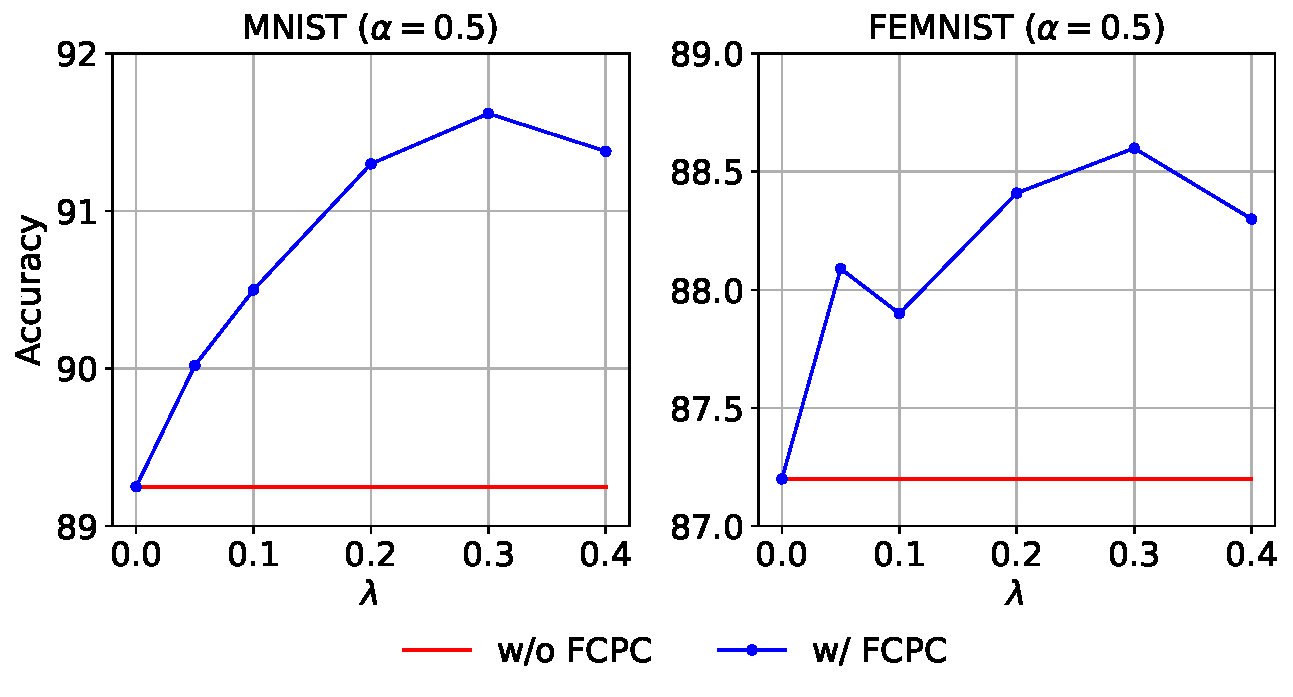
\includegraphics[width=\linewidth]{ablation_study_lambda3.pdf}
    \caption{Ablation studies of \(\lambda\). We set the value of \(\alpha\) to 0.5 and select the MNIST and FEMNIST datasets to conduct experiments with \(\lambda\) taking values from the set \(\{0.1, 0.2, 0.3, 0.4\}\) to explore the appropriate value of \(\lambda\).}
    \label{fig:enter-label}
    }
\end{figure}


\begin{figure*}[t]
    \centering
    \includegraphics[width=0.9\linewidth]{CIFAR10_all_in_one_row.pdf}
    \caption{\textbf{Ablation studies on $\beta$.} We select a value of $\beta$ that is as adaptive as possible to multiple scenarios by comparing the effect of different regularization strengths on model performance on FedAvg.}
    \label{fig:beta}
\end{figure*}


% \paragraph{Coefficient\(\lambda\)}
\textbf{ Coefficient \(\lambda\).} Considering the characteristic of the FedAvg algorithm itself, which performs weighted averaging based on the amount of data, the label skew may play a dominant role. Based on this, we search for the relatively most appropriate value of \(\lambda\) in the set \(\{0.1, 0.2, 0.3, 0.4\}\) to measure the distribution difference between clients. 
As \(\lambda\) gradually increases, the model's adaptability to the data amount difference is enhanced. However, when \(\lambda\) is too large, it may overemphasize the data amount deviation and relatively weaken the impact of the label deviation, causing the model performance to be affected again. \rev{Accordingly, $\lambda=0.3$ is treated as an empirically selected default rather than a theoretically optimal constant. The revised sensitivity study evaluates this choice across client scales and heterogeneity levels, while the Appendix proves only the boundedness and single-skew reduction properties that hold for every $\lambda\in[0,1]$.}



% \paragraph{Coefficient $\beta$}
\textbf{Coefficient $\beta$. }We systematically evaluated the impact of the hyperparameter $\beta$ on FCPC's performance across various data-heterogeneity scenarios (controlled by $\alpha \in \{0.05, 0.1\}$). Experiments were conducted with $\beta \in \{0.05, 0.1, 0.2, 0.3\}$ while keeping all other conditions (network architecture, dataset, training epochs, optimizer settings, and data augmentation) identical.
The results show that FCPC's performance improves with increasing $\beta$, stabilizes, and then slightly declines. Moderate $\beta$ values strengthen regularization, enhancing inter-client gradient consistency and improving performance. Conversely, excessive $\beta$ introduces overly strong constraints that hinder learning, leading to suboptimal performance.
Across all experimental configurations, $\beta = 0.2$ consistently yielded near-optimal results (see Fig. \ref{fig:beta}), representing an ideal balance between constraint strength and learning capacity. This value serves as a robust default when prior information is unavailable.


\begin{table}[htbp]
\caption{Performance comparison of different dissimilarity metrics at $\alpha = 0.5$. JSDN represents the comprehensive indicator of Jensen-Shannon divergence and data size.}
\label{tab:dissimilarity}
\centering
\footnotesize  % IEEE 表格要求使用脚注字号
\begin{tabular}{lcccc}
\toprule
\multirow{2}{*}{Dataset} & \multicolumn{4}{c}{Dissimilarity Metrics} \\
\cmidrule(lr){2-5}
& \textbf{JSDN} & \multicolumn{1}{c}{Jensen-Shannon} & \multicolumn{1}{c}{Euclidean} & \multicolumn{1}{c}{Cosine} \\
& & \multicolumn{1}{c}{divergence} & \multicolumn{1}{c}{distance} & \multicolumn{1}{c}{distance} \\
\midrule
MNIST    & \textbf{91.63} & 90.52 & 90.27 & 90.38 \\
FEMNIST  & \textbf{88.61} & 87.47 & 86.30 & 86.45 \\
CIFAR10  & \textbf{80.08} & 78.52 & 76.75 & 76.70 \\
\bottomrule
\end{tabular}
\label{tab:comparsion of metrics}
\end{table}



% \paragraph{Dissimilarity measures}

\textbf{Dissimilarity measures.} We first validate the effect of the JSDN metric adopted in this paper on the performance of FCPC at \(\alpha\) = 0.5, and then replace the dissimilarity metrics with Jensen-Shannon divergence, cosine distance, and Euclidean distance, respectively, and then present the classification accuracy of the four metrics in a table, as shown in Table \ref{tab:comparsion of metrics}. We observe that our proposed FCPC performs best on the JSDN dissimilarity metric. This preference is attributed to the unique advantage of JSDN to measure both label distribution and quantity distribution.


\subsection{Engineering Applications}
In intelligent transportation systems, the collaborative optimization of traffic signal timing and vehicle route planning relies heavily on the fusion of multi-source IoT data, among which the vehicle-road collaborative network composed of roadside units (RSUs), on-board units (OBUs), and traffic light controllers is a typical application scenario. These IoT devices are distributed in diverse road segments and generate a large amount of non-IID traffic data due to differences in traffic flow density, vehicle types, and travel purposes: for example, RSUs at urban intersections in peak hours mainly collect data with high congestion labels and large sample sizes, while RSUs in suburban roads mostly obtain data with low congestion labels and small sample sizes; OBUs of freight vehicles on highways generate data with stable high-speed characteristics, which are significantly different from the data with frequent start-stop characteristics generated by OBUs of passenger cars in urban areas. 


\begin{figure}
    \centering
    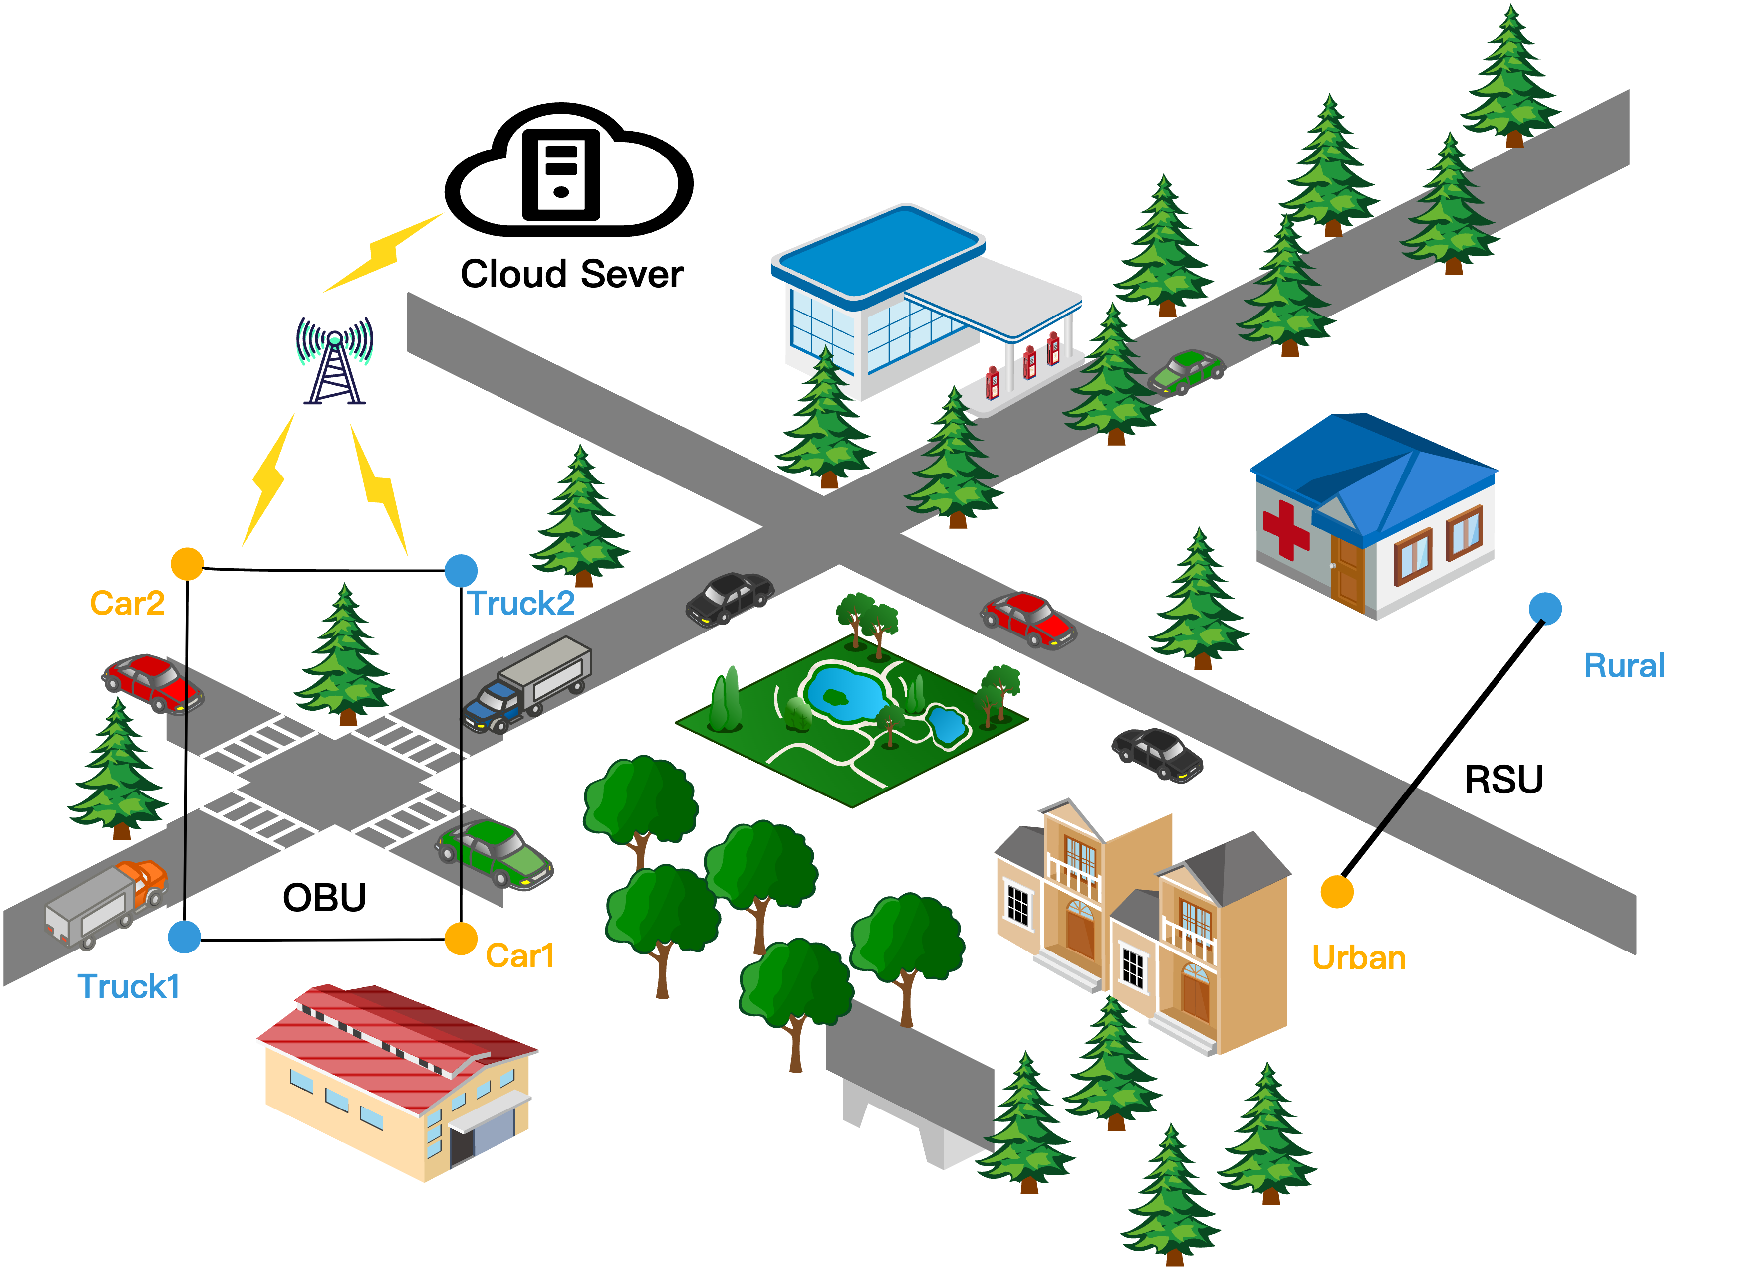
\includegraphics[width=1\linewidth]{IoT2 (1).pdf}
    \caption{The heterogeneous information sources in urban and rural areas form the RSU, while different modes of transportation such as trucks and cars form the OBU, collectively forming the heterogeneous data network of the IoT.}
    \label{fig:placeholder}
\end{figure}

To address this, the FCPC algorithm can be integrated into the intelligent transportation IoT system (see Fig. \ref{fig:IoT}): each RSU, OBU, and traffic light controller acts as a client in federated learning, and first uploads the label distribution  and data size of local traffic data to the cloud server after LDP processing; the server calculates the JSDN matrix based on the uploaded information, and pairs clients with significant differences in data distribution  through the client pairing algorithm; during local training, the paired clients constrain each other through the FCPC regularization term, which reduces the divergence of gradient update directions caused by non-IID data, enables the local models to learn the characteristics of heterogeneous traffic data more comprehensively, and then aggregates the local model parameters to form a global model. This global model can be used to predict short-term traffic flow in each road segment and optimize traffic signal timing dynamically, thereby reducing traffic congestion and improving travel efficiency.

\begin{figure}[h]
    \centering
    \rev{
    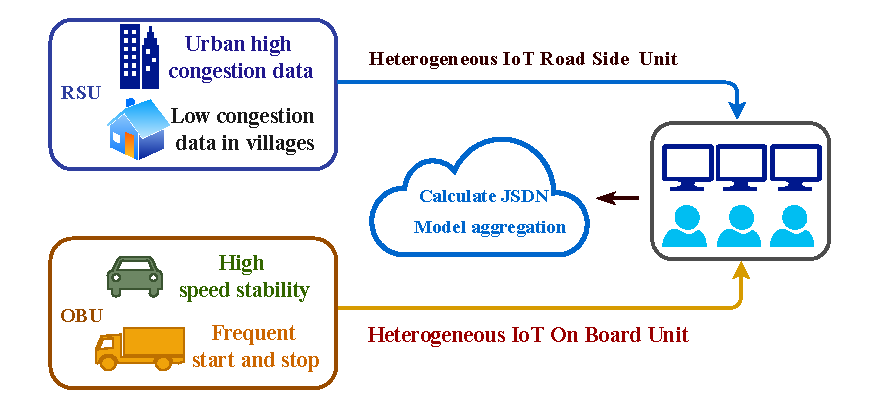
\includegraphics[width=\linewidth]{IoT-revise.pdf}
    \caption{\textbf{FCPC in IoT.} This diagram illustrates the engineering application logic of the FCPC framework in IoT-driven intelligent transportation systems. }
    \label{fig:IoT}
    }
\end{figure}
In practical applications, the plug-and-play nature of FCPC allows new IoT devices to be seamlessly integrated into the federated learning system without modifying the underlying framework, which is highly adaptable to the continuous expansion of intelligent transportation infrastructure. Our subsequent work will focus on applying the FCPC algorithm to the collaborative response of unexpected traffic events, exploring how to use the mutual constraint mechanism between heterogeneous clients to improve the real-time performance and accuracy of event handling, and further enhancing the intelligence level of the transportation system.




% \section{Conclusion and the Future Work}
% In this work, we reveal that participant constraints in IoT federated learning scale directly with data distribution dissimilarity. Motivated by this, we propose FCPC, a novel method that harnesses client correlations to mutually regulate local training.
% To validate its effectiveness and orthogonality, we evaluate FCPC across two network architectures and diverse heterogeneous data scenarios. Experiments on benchmark datasets demonstrate that FCPC consistently outperforms baselines under label skew, quantity skew, and mixed skew.
% This deployable solution addresses real-world IoT challenges where edge devices produce statistically heterogeneous data under resource constraints. FCPC is plug-and-play, imposing minimal computational overhead beyond standard model training. Additionally, we introduce JSDN, a new metric for quantifying client data distribution differences, and design a client pairing algorithm leveraging this metric.
% Future work will target a more general framework to jointly mitigate label/quantity deviations and address broader IoT data heterogeneity.



\section{Conclusion}
\rev{This paper addresses the critical challenge of performance degradation in federated learning (FL) caused by dual-skewed (label and quantity) non-IID data in Internet of Things (IoT) systems. A key insight driving this work is that the mutual constraint potential between clients is positively correlated with their data distribution dissimilarity. Building on this insight, a novel, dissimilarity-aware framework named FCPC is proposed, which comprises two synergistic components: (1) the Jensen-Shannon Divergence and Skew Indicator Number (JSDN) index for precise client heterogeneity quantification, and (2) a client pairing and mutual-constraint mechanism that employs a lightweight regularization term during local training to align gradient updates and mitigate dimensional collapse.}

\rev{Extensive experiments on multiple datasets and network architectures evaluate FCPC's efficacy. Its plug-and-play design leaves the global aggregation rule unchanged, but it is not cost free: the revised evaluation reports the additional local regularization, partner-state storage, and model-transfer bytes alongside accuracy and convergence.}

\rev{Future research will explore: (1) adaptive mechanisms for dynamic parameter tuning in evolving IoT environments; (2) extension to broader heterogeneity types (e.g., feature skew and concept drift); and (3) validation in cross-silo industrial FL scenarios with stringent privacy requirements.}


\bibliographystyle{IEEEtran}
\bibliography{cite}


\end{document}
